\subsection{Data Preprocessing}\label{data_preprocessing}
%The preprocessing stage aims either at processing the initial dataset to reduce its complexity or produces extra information
%about the data. It is an optional step, as some algorithms can directly work on the initial data, as H-BkNNJ, H-BNLJ and 
%H-BRJ \cite{Zhang:2012:EPK:2247596.2247602}.
%Some kNN join methods directly treat the dataset, but some need to threat the transformation of the dataset. 
%\vspace{2pt}
The idea of data preprocessing is to transform the original data to benefit from particular properties. This step is 
done before the partitioning of data to pursue two different goals: (1) either to reduce the dimension of data (2) or 
to select central points of data clusters. 

To reduce the dimension, data from a high-dimensional space are mapped to a low-dimensional space by a linear or 
non-linear transformation. In 
this process, the challenge is to maintain the locality of the data in the low dimension space. In this paper, we focus 
on two methods to reduce 
data dimensionality.
The first method is based on space filling curve. Paper \cite{Zhang:2012:EPK:2247596.2247602} uses $z$-value as space-filling curve. The 
$z$-value of a data is a one dimensional value that is calculated by interleaving the binary representation of data coordinates from the most 
significant bit to the least significant bit. 
%This way, $z$-value data can be organized in a one dimensional order by forming a curve that links data in a zigzag manner.%, shown in Figure \ref{z-value-figure}
%Several shifts of data can be used to reduce information loss (about locality) during the transformation process. %The general process of $z$-value can be seen on figure~\ref{projection_partition_figure}.
%\begin{figure}[t]
%\centering
%\scalebox{0.30}{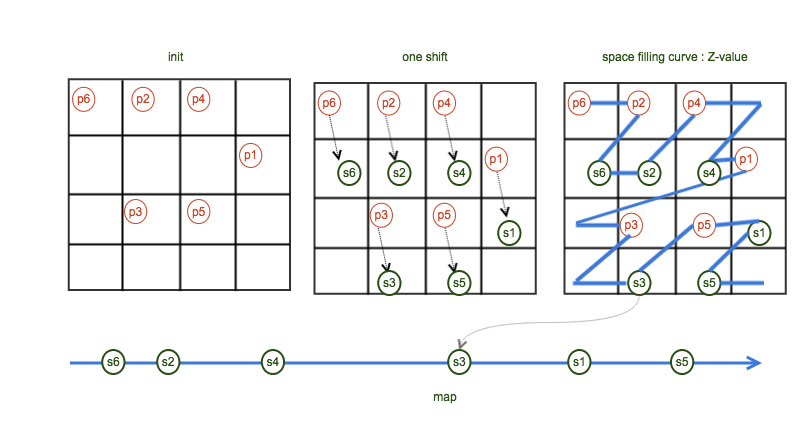
\includegraphics{res/zvalue-final.png}}
%\caption{$z$-value \label{z-value-figure}
%%\caption{$z$-value based partitioning \label{projection_partition_figure}
%}
%\end{figure}
However, due to the loss of information during this process, this method can not fully guarantee integrity of the spatial location of data. 
In order to increase accuracy of this method, one can use several shifted copies of data and compute their $z$-values, although this increases the cost of computation and space. 
The second method to reduce data dimensionality is locality sensitive hashing (LSH) \cite{DBLP:conf/compgeom/2004,Datar:2004:LHS:997817.997857}. This method maps the high-dimensional data into low-dimensional ones, with L families of M locality preserving hash functions $\mathcal{H}$ = $\lbrace$ h(v) =  $\lfloor \frac{a \cdot v + b}{W}\rfloor$ $\rbrace$, where $a$ is a random vector, $W$ is the size of the buckets into which transformed values will fall, and 
$b$ $\in$ $\left[0, W\right]$. %\TODO{rajouter p-stable}
And it makes sure that:
%\TODO{This part is added for explaining the accuracy of LSH later}
\begin{eqnarray}
& if \  d(x, y) \leq d_1, Pr_\mathcal{H}\left[h(x)=h(y)\right] \geq p_1 \\
& if \  d(x, y) \geq d_2, Pr_\mathcal{H}\left[h(x)=h(y)\right] \leq p_2
\end{eqnarray}
where d(x, y) is the distance between two points x and y, and $d_1 < d_2$, $p_1 > p_2$. 
%\TODO{End}

 As a result, the closer two points x and y are, the higher the probability the hash values of these two points h(x) and h(y) in the hash family $\mathcal{H}$ (the set of hash functions used) are the same. 
The performance of LSH (how well it preserves locality) depends on the tuning of its parameters L, M, and W. The 
parameter L impacts the accuracy of the projection: increasing L increases the number of hash families that will be used, it thus increases the accuracy of the positional 
relationship by avoiding fallacies of a single projection, but in return, it also increases the processing time 
because it duplicates data.
The parameter M impacts the probability that the adjacent points fall into the same bucket. The parameter W 
reflects the size of each bucket and thus, impacts the number of data in a bucket.
All those three parameters are important for the accuracy of the result. Basically, the point of LSH for computing $k$NN is to have some collisions to find enough accurate neighbors. On this point, the reference RankReduce paper~\cite{Stupar10rankreduce-} does not highlight enough the cost of setting the right value for all parameters, and show only one specific setup that allow them to have an accuracy greater than 70\%. 

Another aspect of the preprocessing step can be to select central points of data clusters. Such points are called 
\emph{pivots}. Paper \cite{Lu:2012:EPK:2336664.2336674} proposes 3 methods to select pivots. The \emph{Random 
Selection} strategy generates a set of samples, then calculates the pairwise distance of the points in the 
sample, and the sample with the biggest summation of distances is chosen as set of pivots. It 
provides good results if the sample is large enough to maximize the chance of selecting points from different 
clusters. The \emph{Furthest Selection} strategy randomly chooses the first pivot, and calculates the furthest 
point to this chosen pivot as the second pivot, and so on until having the desired number of pivots. This 
strategy ensures that the distance between each selected point is as large as possible, but it is more complex 
to process than the random selection method. Finally, the \emph{K-Means Selection} applies the traditional k-means 
method on a data sample to update the centroid of a cluster as the new pivot each step, until the set of 
pivots stabilizes. With this strategy, the pivots are ensured to be in the middle of a cluster, but it is 
the most computational intensive strategy as it needs to converge towards the optimal solution. The quality of 
the selected pivots is crucial, for effectiveness of the partitioning step, as we will see in the experiments.
%However, the reference PGBJ paper~\cite{Lu:2012:EPK:2336664.2336674} only focuses on one pivot selection 
%and one grouping strategies for evaluating the effect of $k$, of dimension, and of scale. We will experimentally show 
%after that other strategies are also suitable for our dataset.
